\documentclass[10pt]{article}  

%%%%%%%% Preamble %%%%%%%%%%%%
\title{Degree project}
\usepackage[utf8]{inputenc} % File coding uses utf8
\usepackage{amsmath} % Extra commands for math
\usepackage{amssymb} % Math symbols 
\usepackage{graphicx} % Include images in LaTeX
\usepackage{color} % Coloring text
\usepackage{subfigure} % Manage multiple figures
\usepackage{float} % Allow you to use [H] specifier to force the position of the images 
\usepackage{capt-of} % Defines a command \captionof for putting a caption to something that’s not a float.
\usepackage{sidecap} % Defines environments called SCfigure and SCtable (analogous to figure and table) to typeset captions sideways
	\sidecaptionvpos{figure}{c} % Alignment
\usepackage{caption} % to customize the captions in floating environments like figure and table
\usepackage{commath} % Mathematics typesetting support
\usepackage{cancel} % Place lines through maths formulae
\usepackage{anysize} % to set up document margins
\marginsize{2cm}{2cm}{2cm}{0.6cm} % Left, right, up, down
\usepackage{appendix} %Extra control of appendices

% Refereces as links with colors
\usepackage[colorlinks=true,plainpages=true,citecolor=blue,linkcolor=blue]{hyperref}

% Header and Footer
\usepackage{fancyhdr} 
\pagestyle{fancy}
\fancyhf{}
\fancyhead[L]{\footnotesize Blocksworld: Search Algorithms} 
\fancyhead[R]{\footnotesize Foundations of Artificial Intelligence}   
\fancyfoot[R]{\footnotesize 
\includegraphics[scale = 0.35]{images/default-logo.png} \vspace{-1.5cm}}  
\fancyfoot[C]{\vspace{-1cm}\thepage}  % center
% \fancyfoot[L]{\footnotesize Subash Poudyal}  %izquierda
\renewcommand{\footrulewidth}{0.4pt}
\fancypagestyle{firststyle}
{
   \fancyhf{}
}

\usepackage{listings} % To use source code
\definecolor{dkgreen}{rgb}{0,0.6,0} % Color for using code
\definecolor{gray}{rgb}{0.5,0.5,0.5} 
% Language to use
\lstset{language=Matlab,
   keywords={break,case,catch,continue,else,elseif,end,for,function,
      global,if,otherwise,persistent,return,switch,try,while},
   basicstyle=\ttfamily,
   keywordstyle=\color{blue},
   commentstyle=\color{red},
   stringstyle=\color{dkgreen},
   numbers=left,
   numberstyle=\tiny\color{gray},
   stepnumber=1,
   numbersep=10pt,
   backgroundcolor=\color{white},
   tabsize=4,
   showspaces=false,
   showstringspaces=false}

\title{Degree project}

%%%%%%%% Preamble ends %%%%%%%%%%%%

\begin{document}

%%%%%%%%%%%%%%%%%%%%%%%%%%%%%%%% Cover Page %%%%%%%%%%%%%%%%%%%%%%%%%%%%%%%%%%%%%%%%%%%

\thispagestyle{firststyle}
\begin{center}
  \begin{minipage}{0.48\textwidth} \begin{center}
      
\includegraphics[scale = 0.95]{images/default-logo.png}
  \end{center}
    
\end{minipage}
  \vspace*{3cm}
  \vspace*{1cm}
  
\rule{\linewidth}{0.9pt}  \\[1.4cm]
\vspace*{-1cm}
  \textsc{\LARGE School of Electronics and Computer Science}\\[1.5cm]

  \begin{minipage}{0.9\textwidth} 
    \begin{center}
      \textsc{\LARGE Foundations of Artificial Intelligence}
    \end{center}
  \end{minipage}\\[0.5cm]
  \rule{\linewidth}{0.9pt} 
  \vspace*{1cm}

  { \huge \bfseries Blocksworld: Search Algorithms}\\[0.4cm]	
  \vspace*{2cm}
  { \large 
    \emph{Author:} \\	
      Subash Poudyal \\
      sp1g19@soton.ac.uk \\
      28395352 \\
    \vspace*{1.5cm}
    \emph{Moderators:} \\													  
      Dr. Richard Watson \\
      Dr. Enrico Marchioni	\\
  }


  \vspace{3cm} 	

  
\end{center}
																		
\newpage																		
%%%%%%%%%%%%%%%%%%%% Cover page ends %%%%%%%%%%%%%%%%%%%%%%%%%%%%%%%%

\tableofcontents 

\newpage

  \section{Approach}
  \paragraph{} \indent
  After a number of design iterations focusing on the generic code structure to solve the problem along with its adaptability, I settled on the following design. Keep separation of concern in mind, I divided my code structure intro three scripts. One class and the others two merely to make use of that main class: Node. As my favourite programming language and the fact that this problem could be solved with functional-OOP hybrid approach, my language of choosing was Python. Blocksworld is a puzzle that examines the foundations of computer science: data structures and algorithms. Therefore, I’ve not made use of any external libraries making the only dependency python runtime environment itself.

  \subsection{Node}
  \paragraph{} \indent
  Programming a generic structure for the game (the world) was interesting. Although the problem seemed simple, there were a lot of nitty-gritty details to think about such as the size of the grid and starting positions of the blocks; how to make them as adaptable as possible while keeping the core stable enough for an efficient program. For this, I made a class called Node (\textit{Node.py}). Node is the world that the puzzle is contained in. And this world is represented by a 2D array containing the blocks: `A', `B', `C' and asterisk `*'. \\
  
  Although my first thought was to use a single array to store all 16 blocks, I realised it would essentially make no difference in look up times. Dictionaries are the best data structures to go with when it comes to the efficiency of look up times, however, the memory occupied by the dictionary was unnecessarily big. Node class also housed methods such as find\_block, check\_goal\_state and move\_agent.\\

  To solve this puzzle, the agent (empty space) is thought to be an element that moves around the world rather than all other blocks moving their positions. This makes the idea simpler when programming. As python uses `pass by reference' approach, I had to make use of inbuilt library: deepcopy. Node class was my favourite part of the system to code as it housed the integral logics of the Blocksworld. For example, what if the agent was at the bottom right corner and it was asked to move down or right? These logical tasks made designing the class enjoyable.\\

  As an extra, I also made the world adaptable blocked nodes (represented by `X'). i.e. blocks that cannot be moved, increasing or decreasing the difficulty of search in some cases. 


  \subsection{Search}
  \paragraph{} \indent
  Search script is where all the search algorithms are implemented. Unlike Node, this is not a class but just a group of functions. In order to keep things simple yet effective for testing, I implemented search algorithms as independent functions that made use of the Node class. \\
  
  All searches are implemented in a similar way; requiring parameter of the initial / start node. I’ve implemented 7 different searches; 4 tree searches (BFS, DFS, Iterative Deepening and A*) and 3 graph search variants of BFS, DFS and A*. \\

  While all search methods are similar, they make use of different data structures depending on the algorithm to keep efficiency to maximum. BFS uses a queue, a first in first out (FIFO) structure in order to store the nodes and the subsequent children nodes. Although the two algorithms are very similar, DFS on the other hand uses stacks where last in first out (LIFO) is followed. Implementation of IDS was quite easy given the implementation of DFS. IDS is essentially DFS but repeated with a limit on the depth expanded on. \\

  A* search, however, was quite different to all the other searches. While all the others are examples of uninformed searches, A* uses heuristic to navigate its way through to the goal state; better the heuristic, better the performance. To store the nodes, A* uses a priority queue where the nodes in the queue are ordered by their associated value of the heuristic. This is by far the best tree search algorithm amongst the 4 mentioned above. \\ \\
Apart from Node and Search, my only other script is Main where I call functions from \textit{Search.py} in order to solve the puzzle.

  \section{Evidence}
  \paragraph{} \indent
  In this section, I’ll present working evidence of each algorithm going through how the choices were made and briefly explaining how the algorithm works as a whole. Due to some algorithms being less efficient than others in nature, I will be using example with optimal depth of 2 (specification provided initial state to goal state is of optimal depth 14).  It is quite difficult to include all steps (children nodes for each node) in this report, hence, I’ll only be showing few at the start and end respectively. As mentioned before, world is represented by a board containing the blocks: `A', `B', `C' and asterisk `*'. Blank blocks are represented by `0' while the walls are represented by dashes `|'.

  \subsection{BFS and BFS Graph}
  \paragraph{} \indent
  In Breadth First Search, nodes are expanded in the order they’re added to the fringe. On each depth, it’ll expand all nodes and check for goal state, if not found, it’ll move into the next depth repeating this iterative process. Evidence for depth 2 can be seen below. 

  Graph search for BFS would mean that we store the visited nodes and upon each node expansion, we only add nodes to the fringe that have not been visited yet. This makes the search faster.

  \subsection{DFS and DFS Graph}
  \paragraph{} \indent
  Depth First Search always expands the deepest node in the fringe (last added) of the search tree. When goal state is not found, another deepest node is expanded. 

  Similar to BFS Graph, when the visited nodes are stored, search becomes faster; reducing the nodes expanded, trading off space for time. 


  \subsection{IDS}
  \paragraph{} \indent
  Iterative Deepening Search is often used with DFS but with a slightly restricted approach. By limiting the depth in DFS, IDS gradually performs depth-limited DFS increasing the depth until the goal is found. IDS combines the benefits of BFS and DFS.


  \subsection{A* Tree Search and A* Graph Search}
  \paragraph{} \indent
  Unlike other searches mentioned above, A* search is an informed search that combines the cost to reach the node and the cost to get from the node to the goal. A* search is known to be both complete and optimal. 

  To make A* even better, like before, I implemented graph search, storing the nodes that were visited.

  \section{Scalibility}
  \paragraph{} \indent
  In order to study how the algorithms scale as the complexity of the problem grows, I created 13 different initial state; each with different optimal depths ranging from 1 to 13 depths away from the goal state. In order to create these states, I used A* search as it is both optimal and complete, storing a state at each depth until goal state was reached. 

  As most of the search algorithms implemented are random and uninformed, I created a test (Test.py) where all uninformed searches were run 10 times per depth, resulting in 140 runs of each search. Shown below are the states for each depth and in this section, I present results of how increase in depth affects the number of nodes expanded (averaged over the 10 runs). 

  \begin{center}
    \begin{tabular}{cc}
    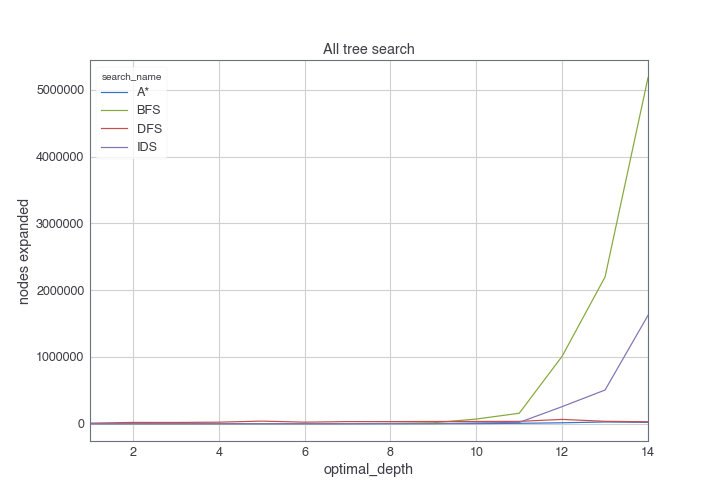
\includegraphics[width=0.65\textwidth]{images/all_tree.png} \\
    \textbf{Figure 4: } All tree searches compared \\
     \end{tabular}
    \end{center}
  
  \begin{center}
    \begin{tabular}{cc}
    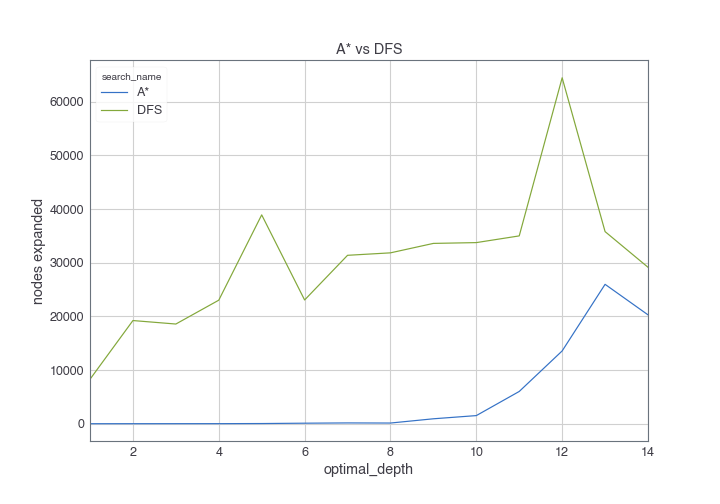
\includegraphics[width=0.65\textwidth]{images/a_star_vs_dfs.png} \\
      \end{tabular}
    \end{center}
  
  \begin{center}
    \begin{tabular}{cc}
    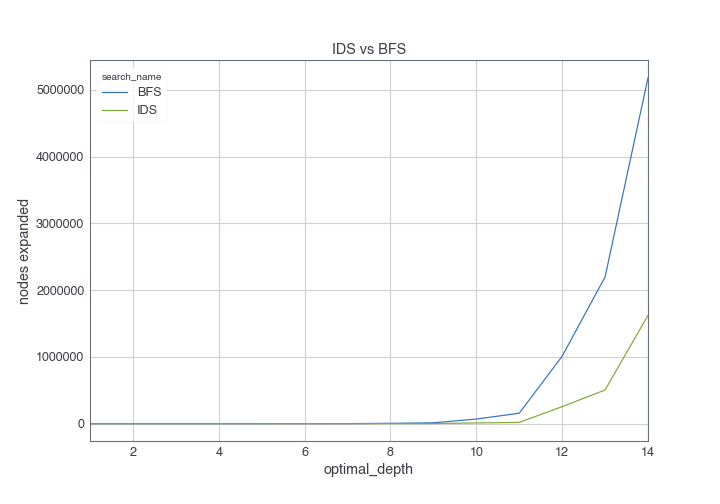
\includegraphics[width=0.65\textwidth]{images/ids_bfs.png} \\
      \end{tabular}
    \end{center}

  \begin{center}
    \begin{tabular}{cc}
    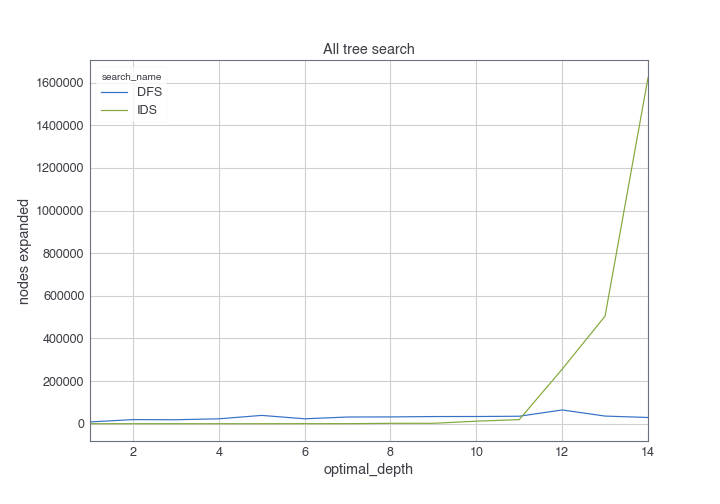
\includegraphics[width=0.65\textwidth]{images/dfs_ids.png} \\
      \end{tabular}
    \end{center}

  \begin{center}
    \begin{tabular}{cc}
    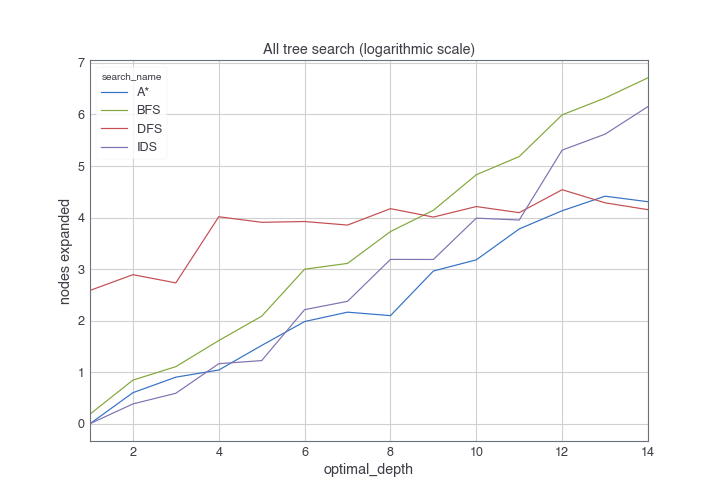
\includegraphics[width=0.65\textwidth]{images/tree_log.png} \\
      \end{tabular}
    \end{center}

  \begin{center}
    \begin{tabular}{cc}
    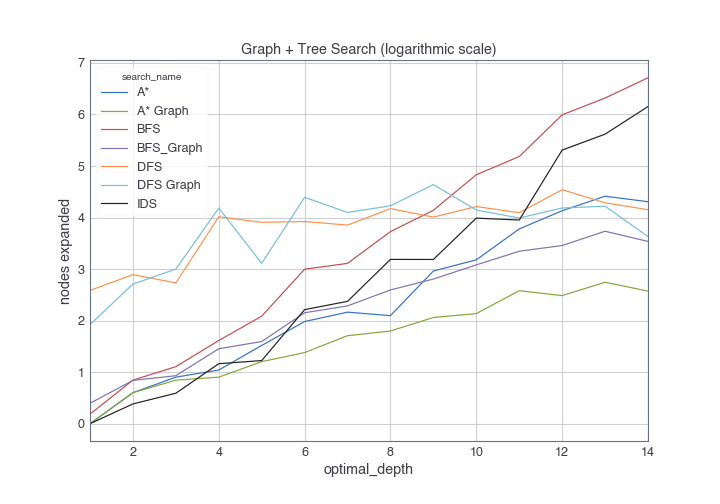
\includegraphics[width=0.65\textwidth]{images/all_logged.png} \\
      \end{tabular}
    \end{center}

  \newpage
  It is clearly visible from figure 4 that after depth 10, BFS and IDS start getting heavily affected by the number of nodes expanded. In other words, their number of nodes expanded starts growing at a very rapid rate. As their number of nodes expanded are so large, we are unable to see the impact on other searches such as A* and DFS. Hence, figure 5 shows the comparisions in node expanded; A* vs DFS. I also created graphs for some more comparisions between graph search and tree search. To visualise the exponential expansion nature of some search methods, I’ve used logarithmic scale for some graphs. Below, I compare different search methods in more detail.

  \subsection{BFS vs IDS}
  \paragraph{} \indent
  From figure 4, we can see that IDS and BFS are the most dominating (in terms of nodes expanded) search methods amongst the others. BFS and IDS are quite similar in terms of performance and this can be seen from the test results as they both follow a close trend; proving that their time complexity is similar. However, although we cannot conclude from the graphs presented above, space complexity of the two algorithms are different. While BFS stores the whole tree, IDS only stores (as an estimate) the branch nodes, making IDS more memory efficient than BFS. 

  \subsection{DFS vs A*}
  \paragraph{} \indent
  Comparing an informed search with uninformed search strategy isn't fair. However, in the search methods explored and implemented, A* approaches the time complexity of DFS around the depth of goal state (depth 14). A* in general has great time and space complexity, however, for this particular problem, the heuristic is not the best. Although I make use of Manhattan distance as the heuristic method, because of the fact that the end position of agent tile doesn’t matter, we cannot have a ``perfect'' heuristic. For this reason, I believe if we were to test A* against DFS for more complex problem (higher depth), DFS may outperform A* search. However,
  from the results observed, A* is clearly better than DFS and for that matter, any other algorithms.

  \subsection{IDS vs DFS}
  \paragraph{} \indent
  From figure 6, we can see that IDS is superior to DFS but that only holds true until depth 11. IDS seems to exponentially grow after the depth of 11 or so. DFS also has a problem; when the search space is large and there is only one solution. These are both not the best search algorithms we have but in this case, DFS seems to be better because of the time complexity (compared to IDS, DFS looks to have constant time).  


  \section{Extras and Limitations}
  \paragraph{} \indent
  If I had more time, I’d have liked to explore the problem further, increasing the depth to more than 14 to compare different search strategies. I’d also include more searches such as bidirectional search and most interestingly, Iterative deepening A* search as it claims to ``keep the memory usage lower than in A*'' \cite{ida*}. In terms of the Blocksworld puzzle itself, I'd have liked if the search problem wasn't limited to a 4 x 4 grid; I'd make the grid adaptable to any sizes. Although heuristics other than Manhattan distance was studied, implementation of Chebyshev distance \cite{chev} was not functional, I'd have loved to expand on that to see the difference in performance against manhattan distance. 

  \section{References}

  \section{Code}
%%%%%%% Bibliografía %%%%%%%%
\bibliographystyle{bst/IEEEtran} 
\addcontentsline{toc}{section}{References}  
\bibliography{bib/IEEEreferences} 
%%%%%%% Bibliografía %%%%%%%%    



\end{document}